\section{\textbf{Simulation}}\label{sec:3}

    The circuit was simulated using PSpice software distributed by OrCAD. The circuit shown in Figure~\ref{fig:schem} was reproduced in PSpice (see Figure~\ref{fig:pspice}). The software does not support the transistor model used in the actual implementation, the TIP31C, instead the Q2N2222 was used to replace it given they are very similar, only the maximum supported values for voltages change. The value of all transistors base resistances was set to $100\:\Omega$. The DC motor simplified equivalent circuit is an inductor and a resistor~\cite{CHAPMAN}. The U8 and U7 times were set to $500\; ms$.\newline
    The motor used in the tests are the one included on the Magician Chassis\footnote{https://www.sparkfun.com/products/retired/12866} by Sparkfun, they have the following characteristics:
    \begin{itemize}
    \item Max Motor Voltage: 6 VDC;
    \item No Load Speed: $90\pm10$ rpm;
    \item No Load Current:190 mA (max.250 mA);
    \item Torque: 800 gf.cm;
    \end{itemize}
	Finally a transient analysis over the circuit was made and the current flowing through the motor is plotted in Figure~\ref{fig:plot_ponteh}. The simulated circuit behavior is exactly the expected, when Q1 and Q3 are activated the current flows... \todo{{FIND THE ROTATION DIRECTION FOR EACH TRANSISTOR PAIR}}

\begin{figure}
\centering
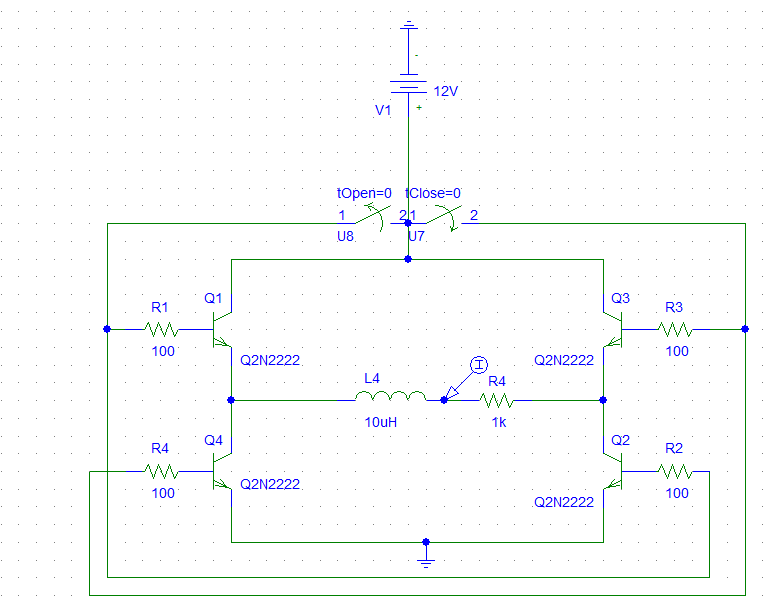
\includegraphics[height=.4\textwidth]{img/schem_pspice.png}
\caption{Schematic on PSpice program.}\label{fig:pspice}%
\end{figure}
	
\begin{figure}
\centering
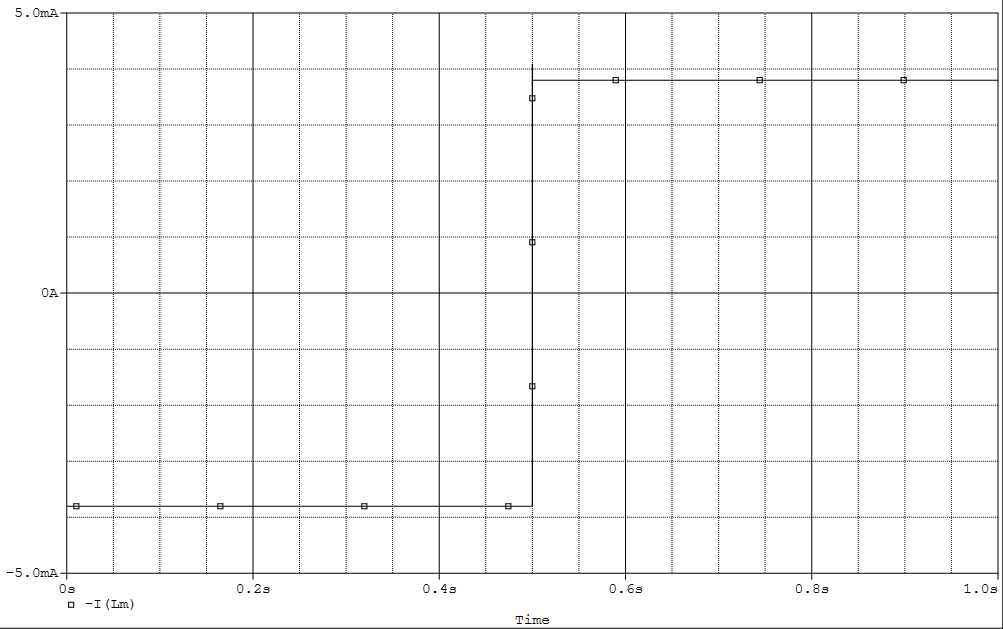
\includegraphics[height=.3\textwidth]{img/plot.png}
\caption{Current x Time} \label{fig:plot_ponteh}
\end{figure}	

\begin{figure}[htp!]
\begin{center}
\begin{circuitikz} %\label{sec:1}
    \draw (2,0) node[npn](q1) at (2,0){}
    (q1.E) node[npn](q4) at (2,-1.55){}
    (q1.E) -- (q4.C);
    \draw (-0.55,0) to[R] (q1.B){};
    \draw (-0.55,-1.55) to[R] (q4.B){};
    \draw (5,0) node[npn,xscale=-1](q3) at (4,0){}
    (q3.E) node[npn,xscale=-1](q2) at (4,-1.55){}
    (q3.E) -- (q2.C)
    (q1.C) -- (q3.C)
    (q4.E) -- (q2.E);
    \draw (3,-2.55) node[ground](gnd){}
    (q2.E) |- (gnd);
    \draw (q3.B)  to[R] (6,0);
    \draw (q2.B) to[R] (6,-1.55);
    % \draw (q1.E) node[elmech]{M}) (q3.E);
    \draw (-0.55,0) -- (-1.0,0) node[circ]{} -- (-1.0,-4) -- (7,-4) -- (7,-1.55) -- (6,-1.55);
    \draw (-0.55,-1.55) -- (-0.80,-1.55) -- (-0.8,-3.5) --(6.5,-3.5) -- (6.5,0) node[circ]{} -- (6,0);
    \draw (3,2) node[spdt,xscale=-1] (s1){}
    (s1.in) |- node[circ]{} (q1.C)
    (s1.out 1) |- (3.5,2.5) |- (7,2.5) |- (6,0)
    (s1.out 2) |- (-1,1.685) |- (-1,0);
    \draw (q1.E) to[sV, color=white, name=M1] (q3.E);
    \mymotor{M1}{0}
    \draw (q2.E) node[circ]{} |- (7.5,-2.31) to[battery] (7.5,1) |- (4,1) |- node[circ]{} (q3.C);
    % \draw (q1.C) --++(0,0.5) node[vcc]{+4.5\,\textnormal{V}};
    % \mymotor{M}{0}
    % \draw (q1.B) -- to[R=100<\ohm>]{};
    % \draw (0,0) node[npn](npn) at (0,0){};
\end{circuitikz}
\caption{H Bridge}\label{fig:schem}%
\end{center}
\end{figure}

